\section{Versuchsaufbau}
\label{versuchsaufbau}

Generelle Netzstruktur, softmax auf Klassen abgebildet
Conv mit MaxPool gefolgt von AveragePool auf Fully Connect auf Softmax

\subsection{Datensätze}
\label{datensaetze}

Die vorgestellten Faltungsmethoden aus Kapitel~\ref{raeumliches_lernen} und~\ref{spektrales_lernen} \bzgl{} des Lernens auf zweidimensionalen euklidischen Graphen wurden über einer Reihe von Datensätzen verifiziert, die im Folgenden vorgestellt werden.
Dafür wurden die Bildermengen in eine Superpixelrepräsentation (\gls{SLIC} und Quickshift) konvertiert und darauf basierend in eine Graphrepräsentation transformiert (\vgl{} Kapitel~\ref{graphrepraesentationen_von_bildern}).
Zusätzlich zu der Präsentation der Datensätze enthält dieses Kapitel damit insbesondere die Parameterwahl der jeweiligen Superpixelalgorithmen, welche jeweils händisch über einer Untermenge der Bilder eines jeden Datensatzes ermittelt wurden, und weiterhin die entsprechenden Merkmalsselektionen, die nach dem beschriebenen Prinzip aus Kapitel~\ref{merkmalsselektion} errechnet wurden.

\paragraph{MNIST}
\label{mnist}

Der \emph{\gls{MNIST}} Datensatz enthält eine große Menge eindeutig klassifizierter handgeschriebener Zahlen von $0$ bis $9$, welcher daher zum Lernen einer Schrift- \bzw{} Zahlenerkennung genutzt werden kann~\cite{mnist}.
Er besteht aus $55000$ Trainingsbildern, $5000$ Validierungsbildern sowie $10000$ Trainingsbildern.
Die Bilder des Datensatzes sind einheitlich auf die Größe $28 \times 28$ skaliert und besitzen lediglich einen Farbkanal mit Grauwerten, welcher angibt, ob ein Pixel des Bildes zu einer Zahl (weiß), zu deren Rand oder zum Hintergrund (schwarz) gehört~\cite{mnist}.
Aufgrund seiner kleinen Datengröße und leichten Handhabung gilt er als die ideale Einführung in Prinzipien des maschinellen Lernens und zeichnet sich damit als ideal für die Verifizierung eines neuen Ansatzes \bzgl{} neuronaler Netze aus.
Insbesondere kann der Datensatz während des gesamten Trainings im Speicher gehalten werden, was den Aufwand \bzgl{} der Verarbeitung und Eingabe der Daten auf ein Minimum reduziert.

Die ermittelten Parameter \bzgl{} der beiden benutzten Superpixelalgorithmen sind in Tabelle~\ref{tab:mnist} gegeben.
Für \gls{SLIC} sind das die Parameter $K \in \gls{N}$, \dhe{} die Anzahl der gewünschten Segmente, sowie $F \in \gls{R}$ für die Gewichtung zwischen der Form und den Farbabgrenzungen der Superpixel.
Für Quickshift ergeben sich dagegen drei wählbare Parameter — $\gls{sigma} \in \gls{R}$ für die Wahl der Standardabweichung der Gaußfunktion, $\alpha \in \gls{R}$ für die Gewichtung des Farbterms sowie $S \in \gls{N}$ zur Einschränkung der Berechnung über ein Fenster der Größe $S \times S$.
Für eine detaillierte Beschreibung der Parameter sei auf Kapitel~\ref{superpixel_verfahren} verwiesen.

\begin{table}[htpb]
\centering
\begin{tabular}{rlrlrlrlrlrl}
  \toprule
  \multicolumn{6}{c}{\gls{SLIC}} & \multicolumn{6}{c}{Quickshift}\\
  \midrule
  $K$: & $100$ & $F$: & $5$ & & & $\gls{sigma}$: & $2$ & $\alpha$: & $1$ & $S$: & $2$\\
  \midrule
  $\overline{N}$: & $10$ & $N_{\min}$: & $10$ & $N_{\max}$: & $10$ & $\overline{N}$: & $2$ & $N_{\min}$: & $1$ & $N_{\max}$: & $2$\\
  $\overline{\gls{degree}}$: & $10$ & $\gls{degree}_{\min}$: & $10$ & $\gls{degree}_{\max}$: & $10$ & $\overline{\gls{degree}}$: & $2$ & $\gls{degree}_{\min}$: & $1$ & $\gls{degree}_{\max}$: & $2$\\
  \bottomrule
\end{tabular}
\caption[Parameterwahl des \gls{MNIST} Datensatzes]{Parameterwahl des \gls{MNIST} Datensatzes}
\label{tab:mnist}
\end{table}

Aus der Wahl der Parameter ergeben sich die ebenfalls in der Tabelle datierten Werte der durchschnittlichen Anzahl an Knoten $\overline{N}$ und deren minimaler \bzw{} maximaler Anzahl $N_{\min}$ \bzw{} $N_{\max}$ sowie dem durchschnittlichen, minimalen und maximalen Knotengrad $\overline{\gls{degree}}$, $\gls{degree}_{\min}$, $\gls{degree}_{\max}$ über der Menge aller aus den Bildern generierten Graphen.
\todo{noch ein satz hierzu}
Abbildung~\ref{fig:mnist} veranschaulicht das Resultat der beiden Superpixel- \bzw{} Graphrepräsentationen eines Bildes aus dem \gls{MNIST} Datensatz.
\section{MNIST}

Trainingsbilder: 55.000

\begin{itemize}
  \item 10.000 Steps mit Batch Size 64 (ungefähr 12 Epochen)
  \item Learning Rate 0.001
  \item klassisches Convolution Neural Network nachgebildet mit Gridgraphen
  \item Conv1: $5 \times 5$, $1 \rightarrow 32$
  \item MaxPool1: Size 2, Stride 2
  \item Conv2: $5 \times 5$, $32 \rightarrow 64$
  \item MaxPool2: Size 2, Stride 2
  \item FC1: 1024
  \item Dropout: 0.5
  \item FC2: 10
\end{itemize}

\subsection{Auswertung}

\begin{itemize}
  \item \textbf{2D Conv > Max:} 0.18s pro Batch, Accuracy: 99.189, Cost: 0.03458
  \item \textbf{2D Conv > 2D Conv > Max:} 0.25s pro Batch, Accuracy: 99.139, Cost: 0.03062
  \item \textbf{Chebyshev $k=25$ GCNN:} 0.91s pro Batch, Accuracy: 98.888, Cost: 0.04329
  \item \textbf{$k=1$ GCNN:} 0.22s pro Batch, Accuracy: 96.765, Cost: 0.10596
  \item \textbf{Partitioned GCNN:}
  \begin{itemize}
    \item Conv > Max: 0.45s pro Batch, Accuracy: 98.998, Cost: 0.03198
    \item Conv > Conv > Max: 2.87s pro Batch, Accuracy: 99.189, Cost: 0.02704
  \end{itemize}
\end{itemize}

\subsection{SLIC}

\begin{itemize}
  \item keine lokale Normierung
  \item Stddev: $1$
  \item 4 Level
  \item Graphkonnektivität: $1$
  \item Anzahl Segmente: $100$
  \item Compactness: $10$
  \item Maximum Iterations: $10$
  \item Sigma: $0$
  \item Anzahl Partitionen: 8
  \item Features: Area, Bbox height, bbox width, Mean Color = $4$ Features
  \item \textbf{Aufbau}: Conv zu 32, Pool2, Conv zu 64, Pool2, Conv zu 128, Pool2, Conv zu 256, Pool2, AveragePool, FC210
  \item Meiste zeit wird durch Partitionierung verschwendet.
  \item \textbf{Ergebnisse}: 0.79s pro Batch, Accuracy: 0,79497, Loss: 0.62814
  \item enttäuschend!
\end{itemize}

\section{PascalVOC}

erster Test:
17 s Preprocess, 12s Training auf BatchSize 64
loss = 0.2, acc = 0.55



% Bei den Datensätzen insbesondere auch die Superpixelalgorithmen erwähnen
% das heißt wie viele Superpixel
% welche Parameter
% mean/max Knotengrad


Merkmalsselektion











% Wie viele Merkmale und welche?


\paragraph{CIFAR-10}
\label{cifar_10}

\cite{cifar_10}

Der \emph{\gls{Cifar}} Datensatz
Er liegt in zwei Versionen vor, \gls{Cifar}-10 und \gls{Cifar}-100, wobei sich diese Arbeit an dem weitaus beliebteren Datensatz \gls{Cifar}-10 bedient.

\begin{figure}[t]
\centering
\subfigure[\gls{SLIC}]{%
  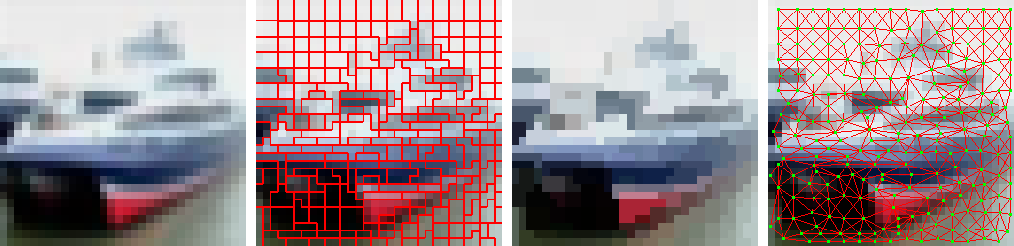
\includegraphics[width=\textwidth]{bilder/cifar_10_slic.png}
}
\subfigure[Quickshift]{%
  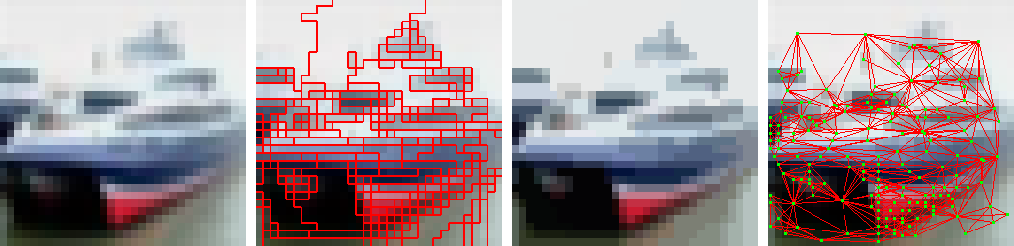
\includegraphics[width=\textwidth]{bilder/cifar_10_quickshift.png}
}
  \caption[\gls{Cifar}-10]{Bild des \gls{Cifar}-10 Datensatzes~\cite{cifar_10}, jeweils dargestellt als (1) Originalbild, (2) Superpixelrepräsentation, (3) Durchschnittsfarbe der Superpixel und (4) Graphrepräsentation.}
\label{fig:cifar_10}
\end{figure}


% \paragraph{Tiny ImageNet}
% \label{tiny_image_net}

% \cite{imagenet}

\paragraph{PASCAL VOC}
\label{pascal_voc}

\emph{\gls{Pascal}} Datensatz
\cite{pascal_voc}

\begin{figure}[t]
\centering
\subfigure[\gls{SLIC}]{%
  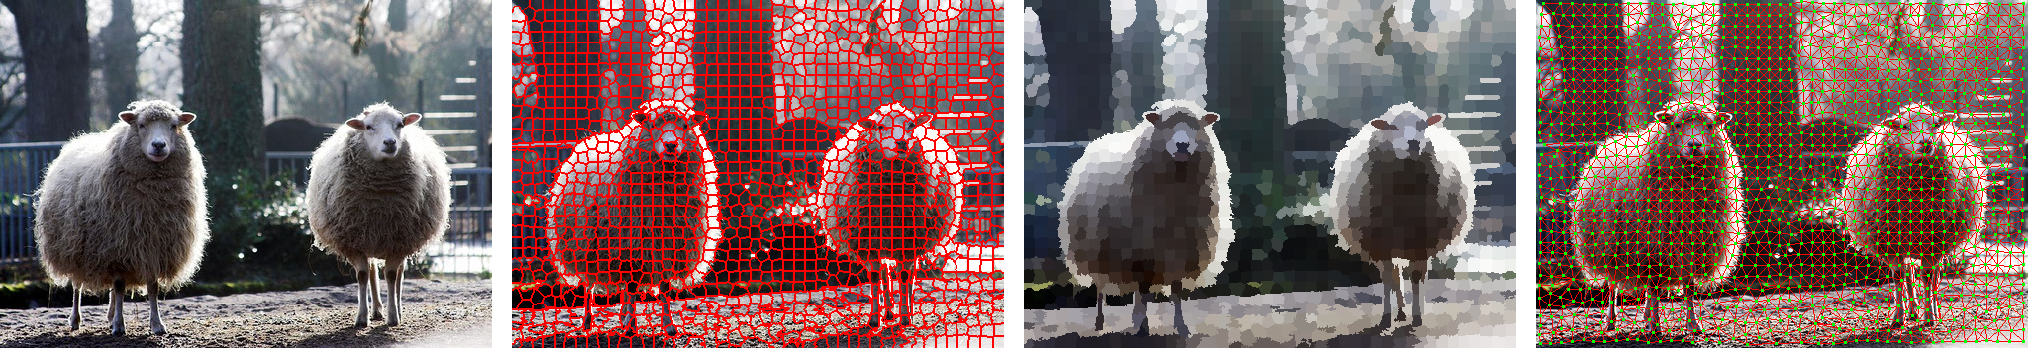
\includegraphics[width=\textwidth]{bilder/pascal_voc_slic.png}
}
\subfigure[Quickshift]{%
  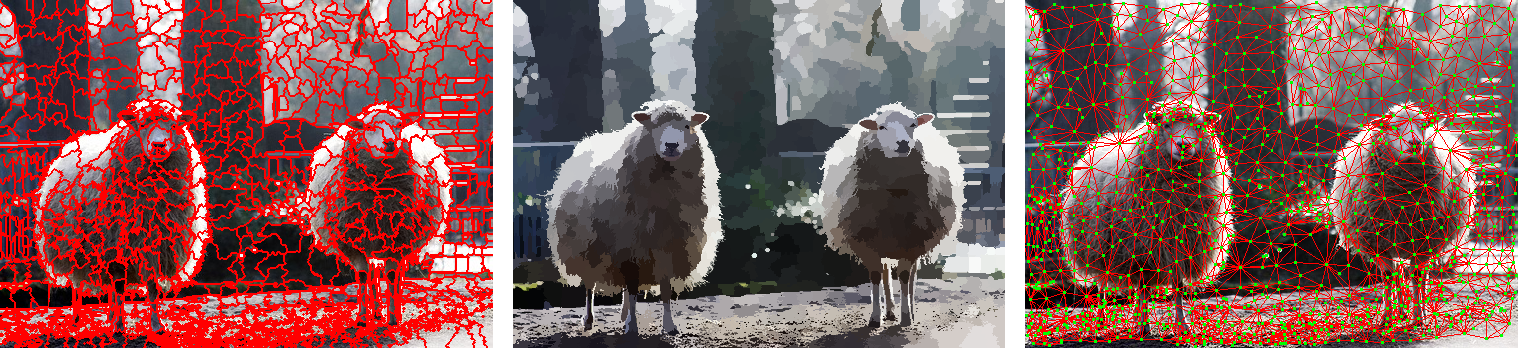
\includegraphics[width=\textwidth]{bilder/pascal_voc_quickshift.png}
}
  \caption[\gls{Pascal}]{Bild des \gls{Pascal} Datensatzes~\cite{pascal_voc}, jeweils dargestellt als (1) Originalbild, (2) Superpixelrepräsentation, (3) Durchschnittsfarbe der Superpixel und (4) generierter Graph.}
\label{fig:pascal_voc}
\end{figure}


\subsection{Metriken}
\label{metriken}

Loss Function
Accuracy

\subsection{Parameterwahl}
\label{parameterwahl}

Vorstellung aller Parameter
Was gibt es denn hier überhaupt?
Dropout, L2 Regularisierung?
BatchSize?
Globale/normale Lokalisierung
Standardabweichung für Gauß
LEARNING RATE, LEARNING RATE DECAY

Alle Faltungen wurden dabei mit einer Partitionsgröße von $8$ bei $K=0$ und $K=1$ implementiert, um ein \gls{CNN} mit einem $3 \times 3$ Filter zu simulieren.
Es erscheint jedoch vorstellbar die Filtergröße bei größerer lokaler Kontrollierbarkeit, \dhe{} $K > 1$, weiter zu reduzieren und die Gefahr des Overfittings damit aufgrund der kleineren Anzahl an Trainingsparametern einzuschränken.

\paragraph{Datenreduktion}
\label{datenreduktion}

\subsection{Augmentierung von Graphen}
\label{augmentierung_von_graphen}

hier auf die Formeln von TensorFlow referenzieren, d.h. TensorFlow Quelle angeben
\cite{tensorflow}

Augmentierung auf Graphen über left/right
Farbanpassungen


nesser ist es, dass Bild vorher zu ändern, da sich dadurch die Superpixelrepräsentation ändert
und folglich zu realisiterischer Augmentierung führt.

\subsection{Vorverarbeitung und Eingabe der Daten}
\label{vorverarbeitung}
